\chapter{Perancangan}
\label{perancangan} 

\section{Struktur Proyek Moodle Mobile}
\label{struktur proyek}

Proyek Moodle Mobile terdiri dari kumpulan file-file dan direktori-direktori utama yang mengandung fungsi dan \textit{source code} untuk aplikasi Moodle Mobile, platform Android dan iOS, alat untuk mebangun perangkat lunak, dan konfigurasi. Struktur dapat dilihat pada Gambar \ref{fig:project-directory}.
\begin{figure} [H]
	\centering  
	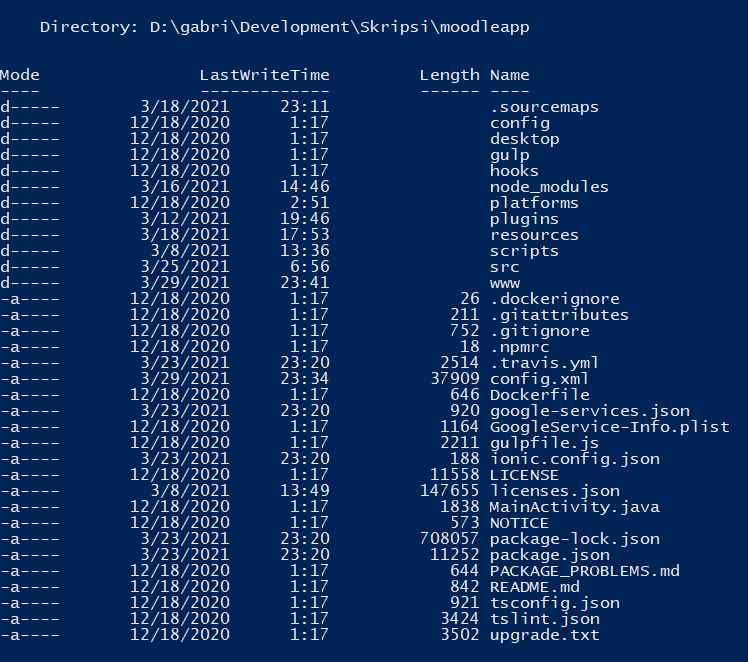
\includegraphics[scale=0.5]{project-directory.PNG}  
	\caption[Struktur direktori proyek Moodle Mobile] {Struktur direktori proyek Moodle Mobile}
	\label{fig:project-directory} 
\end{figure}  

Perubahan pada proyek akan sering dilakukan pada direktori \texttt{src}, dan \texttt{config.xml}. Direktori \texttt{src} berisi kode-kode utama dari aplikasi Moodle mobile dan konfigurasinya. Konfigurasi dari Moodle mobile sendiri diatur oleh file \texttt{config.json} di dalam folder \texttt{src}. File \texttt{Config.xml} berfungsi untuk mengatur konfigurasi dari aplikasi Cordova. Dikarenakan Moodle mobile menggunakan Cordova maka pengaturan saat melakukan \textit{build} untuk perangkat bergerak akan diambil dari file \texttt{Config.xml}. 

Perubahan juga akan terjadi pada direktori \texttt{resources} dan file \texttt{ionic.config.json}. Direktori \texttt{resource} menyimpan sumber untuk ikon dan \textit{splashscreen} yang akan digunakan oleh aplikasi ketika di-\textit{build} untuk platform Android maupun iOS. File \texttt{ionic.config.json} adalah file konfigurasi yang digunakan oleh  Ionic CLI (\textit{Comman Line Interface}), dimana nama aplikasi dan identifikasi aplikasi akan disimpan disana dan dirujuk oleh Ionic CLI ketika digunakan.

\subsection{Perubahan pada \texttt{Config.xml}}
Perubahan pada file \texttt{Config.xml} akan berpengaruh ketika Cordova membangun aplikasi untuk Android dan iOS karena file \texttt{Config.xml} mengatur aturan dan \textit{resource} apa saja yang akan digunakan oleh aplikasi di kedua platform tersebut. 

Perubahan yang dilakukan di dalam file ini adalah sebagai berikut : 

\begin{itemize}
\item Versi aplikasi untuk Android dan iOS.
\item Nama dari aplikasi.
\item Deskripsi aplikasi.
\item Penulis aplikasi.
\item Ikon yang akan digunakan oleh aplikasi dalam platform Android dan iOS.
\item \textit{Splashscreen} yang akan digunakan aplikasi dalam platform Android dan iOS.
\end{itemize}  